\documentclass[../../main.tex]{subfiles}
\begin{document}

{\bf [解答]}

\begin{figure}[htb]
  \centering
  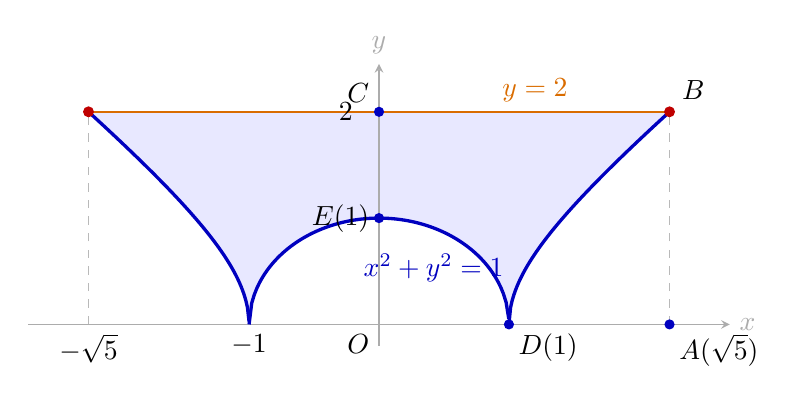
\begin{tikzpicture}[x=1.65cm, y=1.35cm, >=stealth,
      axis/.style={gray!65, thin},
      guide/.style={gray!55, dashed, thin},
    curve/.style={blue!75!black, very thick}]
    % The filled set is bounded above by y=2 and below by the given curve.
    \fill[blue!9] (-2.236068,2) -- (2.236068,2)
    -- plot[domain=2.236068:1, samples=100] (\x,{sqrt(\x*\x-1)})
    -- plot[domain=1:-1, samples=100] (\x,{sqrt(1-\x*\x)})
    -- plot[domain=-1:-2.236068, samples=100] (\x,{sqrt(\x*\x-1)}) -- cycle;
    \draw[axis, ->] (-2.7,0) -- (2.7,0) node[right] {$x$};
    \draw[axis, ->] (0,-0.2) -- (0,2.45) node[above] {$y$};
    \draw[guide] (-2.236068,0) -- (-2.236068,2);
    \draw[guide] (2.236068,0) -- (2.236068,2);
    \draw[orange!85!black, thick] (-2.236068,2) -- (2.236068,2);
    \draw[curve, domain=-2.236068:-1, samples=100]
    plot (\x,{sqrt(\x*\x-1)});
    \draw[curve, domain=-1:1, samples=100]
    plot (\x,{sqrt(1-\x*\x)});
    \draw[curve, domain=1:2.236068, samples=100]
    plot (\x,{sqrt(\x*\x-1)});
    \node[circle, fill=red!75!black, inner sep=1.4pt] at (-2.236068,2) {};
    \node[circle, fill=red!75!black, inner sep=1.4pt] at (2.236068,2) {};
    \node[circle, fill=blue!75!black, inner sep=1.3pt] at (2.236068,0) {};
    \node[circle, fill=blue!75!black, inner sep=1.3pt] at (1,0) {};
    \node[circle, fill=blue!75!black, inner sep=1.3pt] at (0,1) {};
    \node[circle, fill=blue!75!black, inner sep=1.3pt] at (0,2) {};

    % 点ラベル
    \node[below left] at (0,0) {$O$};
    \node[above left] at (0,2) {$C$};
    \node[left] at (0,1) {$E(1)$};
    \node[left=6pt] at (0,2) {$2$};
    \node[above right=1pt] at (2.236068,2) {$B$};
    \node[below right] at (2.236068,0) {$A(\sqrt{5})$};
    \node[below right] at (1,0) {$D(1)$};
    \node[below] at (-1,0) {$-1$};
    \node[below] at (-2.236068,0) {$-\sqrt{5}$};
    \node[orange!85!black, above] at (1.2,2) {$y=2$};
    \node[blue!75!black] at (0.42,0.53) {$x^2+y^2=1$};
  \end{tikzpicture}
  \caption{$y=\sqrt{|x^2-1|}$ と $y=2$ で囲まれる領域（青色）．}
  \label{fig:1971_4_rotated_region}
\end{figure}

$y = f(x)=\sqrt{|x^2 - 1|}$ のグラフは偶関数だから，求める体積 $V$ のうち $x \ge 0$ をみたす部分の体積 $V'$ として
\begin{align}
  V = 2 V' \label{eq:1}
\end{align}
である．絶対値を外すと
\begin{align}
  f(x) &=
  \begin{cases}
    \sqrt{1-x^2} & (0 \le x \le 1)\\
    \sqrt{x^2-1} & (1 \le x)
  \end{cases}
\end{align}
だから，特に$0 \le x \le 1$では$y=f(x)$は円である．
よって$V'$は図のように点を置くと，$\square OABC$から半径$1$の四分円と$y=f(x)$の$[1,\sqrt{5}]$での積分を除いたもので，
\begin{align}
  V'
  &= \square OABC - (\text{四分円}ODE) - (\text{図形}ABD) \\
  &= 4 \sqrt{5}\pi - \dfrac{1}{2} \cdot \dfrac{4}{3}\pi - \int_1^{\sqrt{5}} \pi (x^2 - 1) \, dx \\
  &= \pi \left[ 4\sqrt{5} - \dfrac{2}{3} - \left[ \dfrac{1}{3}x^3 - x \right]_1^{\sqrt{5}} \right] \\
  &= \pi \left[ 4\sqrt{5} - \dfrac{2}{3} - \dfrac{2}{3}\sqrt{5} + \dfrac{2}{3} \right] \\
  & = \pi \left( \dfrac{10}{3}\sqrt{5} - \dfrac{4}{3} \right)
\end{align}
だから，\cref{eq:1}に代入して求める体積は
\begin{align}
  V = \dfrac{4}{3}\pi (5\sqrt{5} - 2)
\end{align}
である．

\newpage

\end{document}
